\documentclass[prl,aps,twocolumn,showpacs,superscriptaddress,longbibliography]{revtex4-1}

%altaffillsymbol
\usepackage{graphicx}% Include figure files
\usepackage{dcolumn}% Align table columns on decimal point
\usepackage{bm}% bold math
%\usepackage{dsfont}
\usepackage{amssymb,amsmath}
\usepackage{sidecap}
\usepackage{wrapfig}
%\usepackage[bookmarks]{hyperref}
\usepackage{natbib}
%\usepackage{braket}
\usepackage{dsfont}


%\bibliographystyle{apsrev}
%\nofiles
\usepackage{graphicx}
\usepackage{leftidx}
%\usepackage[caption=false]{subfig}
%\usepackage{caption}
%\usepackage{subcaption}
\usepackage{color}

\usepackage{bbold} %This package allows to write the identity symbol

\usepackage{wasysym} % In order to introduce polygon symbols in the text
%aus
%\usepackage[geometry]{ifsym}
%\usepackage{amsbsy}
%\usepackage{bbding}
%\usepackage{universal}
%\usepackage{showkeys}


\usepackage{stackrel}

% color for commenting
\newcommand{\col}[1]{\color{red} #1}
% package for strikethrough
\usepackage{soul,xcolor}
\setstcolor{red}



% ENVIRONMENTS
\newcommand{\be}{\begin{equation}}
\newcommand{\ee}{\end{equation}}
\newcommand{\ba}{\begin{align}}
\newcommand{\ea}{\end{align}}
\newcommand{\sysb}{\left\{\begin{array}}
\newcommand{\syse}{\end{array}\right.}
\newcommand{\baa}{\begin{array}}
\newcommand{\eaa}{\end{array}}
\newcommand{\bs}{\begin{split}}
\newcommand{\es}{\end{split}}

\newcommand{\matb}{\left(\begin{array}}
\newcommand{\mate}{\end{array}\right)}


%VERTICAL SPACES
\newcommand{\vsii}{\vspace{2 mm}}
\newcommand{\vsiii}{\vspace{3 mm}}
\newcommand{\vsiv}{\vspace{4 mm}}

% MEASURES
\newcommand{\ddk}{\int \frac{\rmd^{\left( d-1 \right)}k}{\left( 2\pi \right)^{\left( d-1 \right)}}}
\newcommand{\ddq}{\int \frac{d^{ d-1}q}{\left( 2\pi \right)^{\left( d-1 \right)}}}
\newcommand{\Dq}{\int \mathcal{D}q}
%\newcommand{\dd}[2]{\frac{\rmd^{#1}#2}{\left( 2\pi \right)^{#1 }}}
%\newcommand{\ddr}[2]{\frac{\rm{d}^{#1}#2}{\left( 2\pi \right)^{#1 }}}

% GENERIC SHORTHAND
\newcommand{\mal}{\mathcal}
\newcommand{\rmd}{{\rm{d}}}
\newcommand{\rmD}{{\rm{D}}}
\newcommand{\rme}[1]{{\rm{e}}^{#1}}
\newcommand{\mand}{\quad\text{ and }\quad}
\newcommand{\Dim}[1]{\left[ #1 \right]}
\newcommand{\vphi}{\varphi}
\newcommand{\wh}{\widehat}
\newcommand{\wt}{\widetilde}
\newcommand{\ob}{\mal{O}}
\newcommand{\id}{\mathbb{1}}
\newcommand{\trace}[1]{{\rm tr}\left\{ #1 \right\}}
\newcommand{\order}[1]{O\left( #1 \right)}
\newcommand{\ve}{\varepsilon}
\newcommand{\gh}{\phantom}
\newcommand{\EGamma}[1]{\Gamma \lt #1 \rt}
\newcommand{\ha}{\frac{1}{2}}
\newcommand{\eq}{\, = \,}



% SHORTHANDS SPECIFIC TO THE PRESENT TEXT
\newcommand{\pop}[1]{\hat{n}_{#1}}
\newcommand{\bp}{\mathbf{p}}
\newcommand{\bx}{\mathbf{x}}
\newcommand{\brho}{\bm{\rho}}
\newcommand{\brhoo}{\bm{\rho_0}}
\newcommand{\hsi}{\wh{\sigma}}
\newcommand{\whN}{\wh{N}}
\newcommand{\quadblock}[4]{\matb{c|c} #1 & #2 \\ \hline #3 & #4 \mate}
\newcommand{\bE}{{\bf E}}
\newcommand{\bD}{{\bf D}}
\newcommand{\ce}{\rho}
\newcommand{\sdim}[1]{\lqq #1 \rqq}
\newcommand{\tphi}{\widetilde{\vphi}}
\newcommand{\xp}{x_\perp}
\newcommand{\vth}{\vartheta}
\newcommand{\rmn}{{\rm n}}
\newcommand{\rmr}{{\rm r}}
\newcommand{\hatt}{\hat{t}}
\newcommand{\pp}{{\mathbf{P}}}
\newcommand{\tx}{\tilde{x}}
\newcommand{\ty}{\tilde{y}}



% BRACKETS
\newcommand{\lt}{\left(}
\newcommand{\rt}{\right)}
\newcommand{\lqq}{\left[}
\newcommand{\rqq}{\right]}
\newcommand{\lan}{\left\langle}
\newcommand{\ran}{\right\rangle}
\newcommand{\abs}[1]{\left| #1 \right|}
\newcommand{\eval}[1]{\left.\right|_{ #1 }}
\newcommand{\av}[1]{\lan #1 \ran}
\newcommand{\norm}[1]{\left\| #1 \right\|}
\newcommand{\set}[1]{\left\{  #1  \right\}}



% PAULI MATRICES (SIMBOLS AND MATRIX FORMS)
\newcommand{\sx}{{\sigma^x}}
\newcommand{\sy}{{\sigma^y}}
\newcommand{\sz}{{\sigma^z}}
\newcommand{\sxM}{\matb{cc} 0 & 1 \\ 1 & 0   \mate}
\newcommand{\syM}{\matb{cc} 0 & -i \\ i & 0   \mate}
\newcommand{\szM}{\matb{cc} 1 & 0 \\ 0 & -1   \mate}	
\newcommand{\stx}[1]{\widetilde{\sigma}_{#1}^x}
\newcommand{\sty}[1]{\widetilde{\sigma}_{#1}^y}
\newcommand{\stz}[1]{{\widetilde{\sigma}_{#1}^z}}

% NUMBER SETS
\newcommand{\R}{\mathbb{R}}
\newcommand{\N}{\mathbb{N}}
\newcommand{\Z}{\mathbb{Z}}
\newcommand{\C}{\mathbb{C}}

% QUANTUM MECHANICS
\newcommand{\ket}[1]{\left| #1 \ran}
\newcommand{\bra}[1]{\lan #1 \right|}
\newcommand{\bracket}[2]{\lan #1 \right| \!\left. #2 \ran}
\newcommand{\proj}[1]{\ket{#1} \bra{#1}}
\newcommand{\comm}[2]{\left[ #1, #2 \right]}
\newcommand{\acomm}[2]{\left\{ #1, #2 \right\}}




% TRIGONOMETRIC AND HYPERBOLIC FUNCTIONS
\newcommand{\cosa}[1]{\cos \left(  #1 \right)}
\newcommand{\sina}[1]{\sin \left(  #1 \right)}
\newcommand{\tana}[1]{\tan \left(  #1 \right)}
\newcommand{\cossa}[2]{\cos^{#1} \left(  #2 \right)}
\newcommand{\sinna}[2]{\sin^{#1} \left(  #2 \right)}
\newcommand{\tanna}[2]{\tan^{#1} \left(  #2 \right)}
\newcommand{\tann}[1]{\tan^{#1}}
\newcommand{\cosha}[1]{\cosh \left(  #1 \right)}
\newcommand{\sinha}[1]{\sinh \left(  #1 \right)}
\newcommand{\tanha}[1]{\tanh \left(  #1 \right)}
\newcommand{\cossha}[2]{\cosh^{#1} \left(  #2 \right)}
\newcommand{\sinnha}[2]{\sinh^{#1} \left(  #2 \right)}

% OTHER FUNCTIONS
\newcommand{\loga}[1]{\log \lt #1 \rt}
\newcommand{\lna}[1]{\ln \lt #1 \rt}
\newcommand{\BK}[2]{K_{#1} \lt #2 \rt}
\newcommand{\Prob}{\mathbb{P}}


\newcommand{\nol}{\nonumber \\}


\newcommand{\reff}[1]{(\ref{#1})}
\newcommand{\note}[1]{{\bf \small #1}}

% BOUNDS
\newcommand{\maxx}[2]{\max\limits_{#1}^{} \left\{ #2 \right\}}
\newcommand{\minn}[2]{\min\limits_{#1}^{} \left\{ #2 \right\}}

% LIMITS IN SUMS, INTEGRALS, AND THE LIKE
\newcommand{\prodl}[2]{\prod\limits_{#1}^{#2}}
\newcommand{\suml}[2]{\sum\limits_{#1}^{#2}}
\newcommand{\intl}[2]{\int_{#1}^{#2}}
\newcommand{\bol}[2]{\bigotimes\limits_{#1}^{#2}}
\newcommand{\liml}[1]{\lim\limits_{#1}}



% CORRECTIONS
\newcommand{\change}[1]{\textcolor{blue}{#1}}
\newcommand{\changer}[1]{\textcolor{red}{#1}}
\newcommand{\changeg}[1]{\textcolor{green}{#1}}
\newcommand{\changeb}[1]{\textcolor{blue}{#1}}
\newcommand{\tochange}[1]{\textcolor{magenta}{#1}}
\newcommand{\nochange}[1]{\textcolor{black}{#1}}
\newcommand{\mm}[1]{{\tochange{\footnotesize{\bf (#1)}}}}
\newcommand{\ag}[1]{{\footnotesize \changer{#1}}}
\newcommand{\jm}[1]{{\footnotesize \changeg{#1}}}
\newcommand{\comma}{\quad , \quad}

\newcommand{\dar}{\downarrow}
\newcommand{\uar}{\uparrow}


\newcommand{\transp}{\mathtt{T}}


\newcommand{\ind}{b}
\newcommand{\indd}{c}


\usepackage{amsthm}
\newtheorem{mydef}{Definition}
\newtheorem{prop}{Proposition}
\newtheorem{theorem}{Theorem}


 \newcommand{\up}{\uparrow}
 \newcommand{\uu}{\up\, \up}
 \newcommand{\down}{\downarrow}
 \newcommand{\dd}{\downarrow\, \downarrow}

  \newcommand{\tspace}{\rule{0pt}{2.6ex}}
  \newcommand{\norml}{\textnormal}
  \newcommand{\op}[1]{\mathrm{\hat{#1}}}

\begin{document}

\title{Lieb ladders and Rydberg rungs}

\author{us}
\affiliation{School of Physics and Astronomy, University of Nottingham, Nottingham, NG7 2RD, UK}
\affiliation{Centre for the Mathematics and Theoretical Physics of Quantum Non-equilibrium Systems,
University of Nottingham, Nottingham NG7 2RD, UK}



\begin{abstract}
%Rydberg lattice gases under so-called facilitation conditions can be implemented and studied on the most recent manifestations of cold atom quantum simulators. Facilitation introduces a constraint which yields a Hilbert space structure that allows the mapping of many-body states onto an artificial (or synthetic) lattice. These lattices feature in general one or several 
%at bands and thus support immobile localized states. We investigate this in detail for the simple case of a Rydberg ladder. We demonstrate that correlated disorder | imposed by the uncertainty of the atomic positions within the lattice sites | leads to the localization of the many-body wave function and an unusual scaling of the localization length with the disorder strength. Moreover, we show that immobile localized many-body states, which can be prepared experimentally, display a non-monotonic delocalization-localization behavior as the disorder strength is increased.
We study the physics of Rydberg lattice gases under a so-called facilitation condition, inspired by recent advances in the manipulation of optical tweezer arrays. The facilitation mechanism induces constraints on the connectivity of the Hilbert space, resulting in a highly-simplified structure. When combined with the real space geometry of the tweezer array, it allows the realization of synthetic lattices, where individual sites correspond to many-particle ``Fock'' states. These lattices generically feature the presence of flat bands. We exemplify our construction considering a Rydberg ladder (two close-by linear chains). This maps to a synthetic 1D Lieb lattice, whose flat band supports immobile localized states. We analyse the scaling behaviour of the localization, including anomalous scaling at the band edges, for the correlated disorder imposed by the uncertainty of the atomic positions. Finally, we show how these immobile localized states behave under the influence of increasing disorder, which could in principle be tested in an experiment. 
%that the immobile localized many-body states, for which we describe a preparation scheme, display a non-monotonic delocalization-localization behavior as the disorder strength is increased.
\end{abstract}
\pacs{}
\maketitle


Over the past few decades, consistent advances in the manipulation of cold and ultra-cold atomic gases made them into a suitable candidate for a versatile quantum simulation platform \cite{Bloch_2008,Bloch_2012}. Indeed, several paradigmatic many-body models have been recreated and studied experimentally, including the Luttinger liquid \cite{hofferberth2007}, Tonks-Girardeau gas \cite{kinoshita2004}, Bose-Hubbard \cite{greiner2002, greiner2003}, and Fermi-Hubbard \cite{Kohl2005}, permitting to directly observe several predicted phenomena, such as quantum revivals \cite{greiner2002_revival}, Lieb-Robinson bounds \cite{cheneau2012}, and topological phase transitions \cite{hadzibabic2006}.

A particular platform, renowned for featuring considerably strong interactions, is given by Rydberg atoms \cite{a_Saffman_RMP_10, Low_2012, Gallagher_1994}. These are atoms whose valence electrons are excited to high-lying orbitals, leading to a noticeably-enhanced polarizability and, consequently, very strong dipole-dipole or van-der-Waaks interatomic forces. These systems are now employed for a variety of tasks, ranging from quantum information processing \cite{Jaksch2000,Weimer_2010,Saffman_2016}, to the realization of quantum spin Hamiltonians \cite{Labuhn_2015} and their ground states \cite{Schauss_2015}. A hallmark, characteristic feature of Rydberg atoms is that, even at mesoscopic interatomic distances of a few micrometers, the interaction potentials are still strong enough to shift the atomic levels --- and, therefore, the corresponding transitions --- sufficiently out of resonance with an external electromagnetic field to effectively decouple the atoms from it. This gives rise to a correlated production of excitations leading to a rather rich phenomenology \cite{Weimer2010, Lan2016, Levi2016, Lan2015, Schempp2014, Schauss_2015, Low2009, Sibalic2016, Carr2013, Marcuzzi2014, Gutierrez2015}.


The so-called \emph{facilitation} (or \emph{anti-blockade}) mechanism \cite{Ates_2007,Amthor_2010,Garttner_2013,schonleber2014,Lesanovsky_2014,Urvoy_2015,Valado_2016} emerges upon shining an off-resonant laser on an ensemble of Rydberg atoms. The interactions can then shift the atomic transitions closer to resonance so that atoms at a certain distance from an excited one couple to the laser field and can undergo (de-)excitation. This mechanism therefore translates the global action of the laser on the sample into a local transfer of excitations. This is at the basis of interesting connections to the physics of glasses \cite{Lesanovsky2013} and population dynamics \cite{CPE2017,Marcuzzi2016,Buchhold2017}, but more fundamentally constitutes a form of transport.


In quantum systems, it is well-established that transport can be heavily affected by the presence of quenched disorder, a phenomenon known as Anderson localization \cite{Anderson1958}. In the presence of randomly-distributed impurities in a metal, for example, different paths taken by an electron can interfere destructively, leading to localization , i.e., the electron's wave function is not a Bloch wave extending over the whole system any longer, but spatially localized instead. In one and two dimensions, this effect is so relevant that for arbitrarily small disorder all wavefunctions are localized and transport is effectively impossible \cite{Mott1961,Ishii1973}. Since their first prediction, these effects have been experimentally observed in a range of systems, spanning electron gases \cite{Cutler:1969}, cold atoms \cite{Billy:2008,Roati:2008,Semeghini:2015}, thin films \cite{Liao:2015} and periodically-driven nitrogen molecules \cite{Bitter:2016}. Besides quenched disorder, localized states can also arise in tight-binding models from particular lattice geometries. In these cases, destructive interference leads to the emergence of flat bands. Models with flat bands typically allow the construction of localized eigenstates, and have been experimentally realized with cold atoms \cite{Shen2010}, photonic lattices \cite{Mukherjee2015}, and synthetic solid-state structures \cite{slot2017, drost2017}. When disorder is introduced in such systems, these pre-existing localized states couple to the dispersive, system-spanning ones and start acting like scatterers, inducing a richer phenomenology, such as localization enhancement \cite{Leykam2017}, Anderson transitions in lower-dimensional systems \cite{Bodyfelt2014}, and disorder-induced delocalization \cite{Goda2006}. 

In this work, we show how Rydberg gases can also act as quantum simulators for disordered models with flat bands, opening the opportunity to access these phenomena in current experiments. In particular, the advanced control of optical tweezer arrays permits the creation of various lattice geometries \cite{Nogrette_2014, Barredo2017} close to unit filling \cite{Barredo_2016,Endres_2016}. 
% Importantly, techniques allowing for addressing a single atom in such arrays have been developed \cite{Labuhn_2014,Bloch_2016,Greiner_2009,Zwierlein_2015}


\emph{Model---} We start by considering a regular (not necessarily cubic) lattice of $N$ optical tweezers, each loaded with a single Rydberg atom, and with nearest-neighbor distance $R_0$. A laser is shone with a frequency close, up to a detuning $\Delta$, to an atomic transition between the electronic ground state $\ket{\down}$ and a Rydberg level $\ket{\up}$. In a simplified picture, the atoms can thus be described as effective two-level systems. Atoms in the Rydberg state $\ket{\up}$ lying at a distance $D$ from each other interact, if not too close, via an algebraically-decaying potential $V(D) = C_\alpha / D^\alpha$, with $\alpha = 3$ for dipole-dipole interactions and $\alpha = 6$ for van-der-Waals ones. For simplicity, we set $C_\alpha > 0$; all the considerations made below can be replicated for $C_\alpha < 0$ by changing the signs where appropriate. Transforming to the frame rotating with the laser frequency and discarding counter-rotating terms (rotating wave approximation), the system can be described by the Hamiltonian 
%
\begin{align}
 \op{H} = \Omega \, \sum_k^N  \op{\sigma}_x^{(k)} \, + \, \Delta\, \sum_k^N\,\op{n}_k +\,  \,
 \sum_{\substack{k= 1\\ m \ne k}}^N \, V(D_{km}) \, \op{n}_m\, \op{n}_k,
 \label{Eq:Hamil_full}
\end{align}
%
where we set for convenience $\hbar=1$, $\Omega$ is the laser Rabi frequency, $k$ and $m$ are lattice indices, $D_{km}$ denotes the distance between atoms in sites $k$ and $m$, $\op{\sigma}_x^{(k)} = \ket{\up_k} \bra{\down_k} + \ket{\down_k} \bra{\up_k}$ and $\op{n}_k = \proj{\up_k}$. The facilitation (or anti-blockade) condition is obtained by setting $\Delta = -V(R_0)$, so that an isolated excited atom makes its neighbors resonant with the laser. In the following, we assume $\abs{\Delta} \gg \Omega$, so that non-facilitated atoms are sufficiently off-resonant to neglect their excitation. Furthermore, denoting by $R_1$ the distance between next-nearest neighbors, we set $V(R_1) \gg \Omega$ as well. This last condition implies that an isolated excitation can facilitate the production of another on a neighboring site, but no additional one can then be produced in the neighborhood, as the process is energetically suppressed. For example, in one dimension $\abs{\bra{\up \up \up} \rme{-iHt} \ket{\up \up \down}}^2 \sim O((\Omega / V(R_1))^2)$. In the following, we neglect these transitions, effectively splitting the Hilbert space into subspaces separated by energy scales $\gg \Omega$ . Each subspace comprises a set of quasi-resonant states separated by scales $\sim O(\Omega)$ (see Ref.~\cite{a_Marcuzzi_PRL_17} for more details on this structure). From a simple perspective, this means that a single excitation can at most produce one more in the neighborhood, after which either the former facilitates the de-excitation of the latter, or vice versa. Starting from a state with a single excitation, the relevant Hilbert subspace will consist of all states with either a single excitation or a single pair of excitations on neighboring sites. This draws a lattice structure in the Hilbert space which closely resembles the original geometry of the tweezers, according to the following basic rules, sketched in Fig.~\ref{Fig:flat_band_lattices} for a few planar examples:  
\begin{figure}
% 	    

	      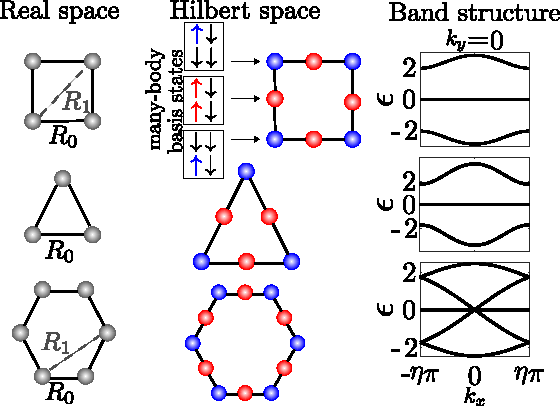
\includegraphics[width=0.5\textwidth]{graphics/lattices_real_hilbert_bands.pdf}

    %
		\caption{
		    First column: geometry of a square, a triangular, and a hexagonal lattice 
		    in real space. The blue spheres give the position of the Rydberg atoms and
		    the lines the interaction between neighboring atoms. Second column: respective lattices in Hilbert 
		    (for $\Delta = -V_{NN}$). The blue dots represent the main state with a single excitation while the red spheres
		    are intermediate state corresponding to a single pair of neighboring excitation.
		    Third column: two cuts of the band structure for each lattice geometries at $k_y= 0$ (left) and $k_y = \pi$ (right).
		    The green bands are the flat bands of the respective lattice. The red and blue bands are the dispersive bands of the system
		    (different colors for easier readability).
		    %
                    }
  
	\label{Fig:flat_band_lattices}
\end{figure} 
%%
%%
%%
(i) in the original lattice structure, draw the links joining nearest neighbors; (ii) each site can now be identified with the state having a single excitation on that site. This exhausts all ``one-excitation'' states in the subspace; (iii) each ``pair'' state can be straightforwardly associated to the link joining the two excited atoms; hence, place an additional site in the midpoint of each link and associate it with the corresponding ``pair'' state. The links in this new-found structure now effectively represent pair of states connected by the Hamiltonian, which can be therefore seen as a tight-binding model on a generalised lattice. In the case of a square lattice, the new structure (see Fig.~\ref{Fig:flat_band_lattices}) is called \emph{Lieb lattice} and is known to feature a flat band and two dispersive ones which meet with a cone-like structure at the edges of the first Brillouin zone. However, this construction is general and can be extended to any kind of ``regular'' lattice \footnote{We use here the term ``regular'' in a loose sense to denote lattices whose primitive lattice vectors all have the same length.}. Most of these structures will also support flat bands. It can be shown \cite{SM} that, calling $n_1$ ($n_2$) the number of one-excitation (pair) states in a unit cell, the number of flat bands $n_{flat}$ must be $\geq \abs{n_1 - n_2}$. For the examples of Fig.~\ref{Fig:flat_band_lattices}, the square lattice has $n_1 = 1$, $n_2 = 2$, $n_{flat} = 1$, the triangular lattice $n_1 = 1$, $n_2 = 3$, $n_{flat} = 2$ and the honeycomb lattice $n_1 = 2$, $n_2 = 3$, $n_{flat} = 1$. 

Disorder enters the picture through the uncertainty in the atomic positions: the optical tweezers are not, in fact, infinitely narrow and there is an intrinsic uncertainty in the atomic positions. Due to the noticeable amplitude of the interaction potential, even small displacements from the centre of the traps can significantly shift the atomic transitions off resonance from the laser frequency, thereby hindering the facilitation mechanism, as studied e.g.~in Ref.~\cite{a_Marcuzzi_PRL_17}. In fact, the interaction potential seen by an atom at a distance $R = R_0 + \delta R$ from an excitation will be $V(R) = V(R_0 + \delta R) \equiv V(R_0) + \delta V$; note that, since $V(R) >0$, $\delta V > - V(R_0)$, i.e.~the energy shifts are only defined on a domain $[-V(R_0), +\infty)$. At small disorder ($\delta R \ll R_0$) they can be approximated by $\delta V \approx -\alpha C_\alpha / R_0^{\alpha + 1} \delta R$. These energy shifts are random and only affect pair states, creating a disordered potential landscape over the pair (red) sites in Fig.~\ref{Fig:flat_band_lattices}. The single-excitation (blue) sites' energy remains unvaried instead, which in particular implies that any eigenstates of the tight-binding Hamiltonian which exclusively have component on these sites will be unaffected by disorder, and remain eigenstate of the disordered Hamiltonian at the same energy for any random realization. Note, however, that for the Hilbert space structure to be maintained, the disorder strength cannot exceed the scale of energetic suppression fixed before, i.e.~$\delta V \ll V(R_1)$. 

In order to characterize the disorder, we denote by $\omega$ the optical trapping frequency (assumed hereafter to be isotropic in space), by $m$ the atomic mass and by $T$ the temperature. The probability distribution of a trapped atom can then be approximately described as a Gaussian of width $\sigma$ around the trap centre. We require now that (I) $k_B T \gg \hbar \omega$: this implies that one can use the semiclassical estimate $\sigma \approx \sqrt{k_B T / m\omega^2}$ and moreover that the thermal de Broglie wavelength of the atom is much smaller than the distribution width. In other words, the atom can be approximately considered localized somewhere within the trap according to a classical probability distribution. (II) $\omega \Delta t \ll 1$, with $\Delta t$ the duration of an experiment: this ensures that the atoms will not appreciably move from their positions in this time frame and thus the disorder is quenched. (III) $\Omega \gg \omega$, or in other words the dynamics of the internal degrees of freedom is much faster than the one of the kinetic ones, so that within an experiment one can probe the action of the disordered Hamiltonian on the system while keeping the disorder quenched (i.e.~fixed). As pointed out in Ref.~\cite{a_Marcuzzi_PRL_17}, while the positions of the atoms are picked from independent Gaussian distributions, the energy shifts depend on them via the distances $D_{km}$. This produces a correlated distribution $P(\delta V_{km} ,\, \delta V_{m l}) \neq P(\delta V_{km}) P(\delta V_{ml})$. 
%The correlated nature of the distribution of energy shifts can also be inferred from the triangular inequality: since $D_{km} + D_{ml} \geq D_{kl}$ then, using the approximate expression for $\delta V \ll V(R_0)$ shown above one finds $\delta V_{kl} \geq \delta V_{km} + \delta V_{ml} - \alpha V(R_0)$. For weak disorder, this constraint is satisfied most of the times (since $\delta V \geq - V(R_0)$ by construction) which suggests that these correlations do not play any major role. 
A more detailed discussion of the properties of the probability distribution of energy shifts can be found in \cite{SM}; here we just remark that this distribution is fat-tailed, i.e.~it has no well-defined moments; however, for weak noise its algebraically-decaying tails are suppressed to a point where they could not be probed in any reasonable simulation or experiment.


In the remainder of our discussion, we shall focus on a ladder configuration, i.e.~a quasi-one-dimensional lattice formed by placing two linear chains parallel to each other at a lattice spacing distance $R_0$. For this example, the artificial lattice (corresponding to the ``1D Lieb lattice'' case of Ref.~\cite{Leykam2017}) in the Hilbert space is sketched in Fig.~\ref{Fig:decoupling}(a). The unit cell consists of five sites with $n_1 = 2$ and $n_2 = 2$ and the band structure features one zero-energy flat and four dispersive bands grouped in two pairs of opposites (panel (d)). 
%%%
%%%
%
\begin{figure}
% 	    

	      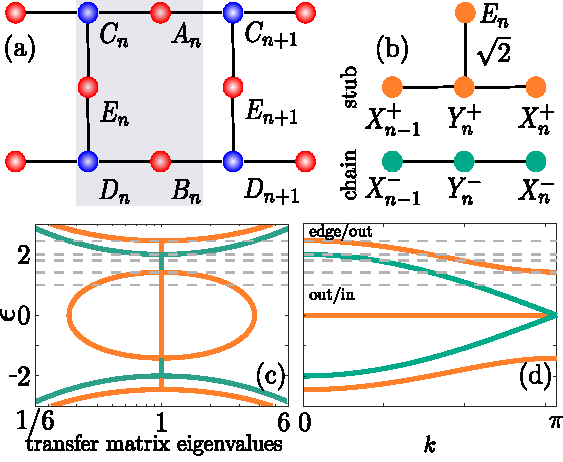
\includegraphics[width=0.5\textwidth]{graphics/decoupling.pdf}

    %
		\caption{(a) One dimensional Lieb ladder. Blue spheres correspond to the main states (singly excited states) and red spheres represent intermediate state
		(doubly excited states). (b) Lieb lattice after the detangling procedure introduced in \cite{a_Flach_EPL_14,Leykam2017}.
		     (c) Eigenvalues of the transfer matrix in the case of no disorder.
		     The dotted lines corresponds to the energies $\epsilon = \{0,1, \sqrt 2, 1.8, 2, \sqrt 6\}$ at which the scaling of the localization lengths is determined.
                    (d) Band structure of the Lieb ladder without disorder. The bands corresponding to the stub lattice are given in red and bands of the ordinary 1D chain are shown in blue.
                    }
  
	\label{Fig:decoupling}
\end{figure}  
%
%
%%%
%%%
Via a detangling transformation \cite{a_Flach_EPL_14,Leykam2017} this lattice (before the introduction of disorder) can be mapped onto a pair of disjoint ones (see Fig.~\ref{Fig:decoupling}(b)), a chain (in blue, supporting the two innermost dispersive bands) and a stub lattice (in red, supporting the flat and two outermost dispersive bands) \cite{SM}. The states of the flat band can be classified into a macroscopic set of localized ones (of the form $(\ket{A_n} + \ket{B_n} - \ket{E_n} - \ket{E_{n+1}})$) with support exclusively on pair sites plus an extended one (of the form $\sum_n (-1)^n (\ket{C_n} - \ket{D_n})$) with support exclusively on single-excitation sites. The latter is insensitive to the disorder and survives unaffected to its introduction. 

A similar model was studied in Ref.~\cite{Leykam2017}, where however the disorder was generated independently on each site. In order to assess how much the localization properties may be affected by having no disorder on half of the lattice sites, we start by performing an analogous study of the scaling properties of the \emph{localization length} $\xi$ at small disorder. This quantity describes, at fixed energy $E$, the exponential envelope of eigenstates of the disordered Hamiltonian; in other words, wave functions are peaked and mostly concentrated in a specific area of the lattice and decay as $\rme{-x/\xi}$ with the distance $r$ from it. For every value of the energy, it is possible to extract two distinct values of the localization length, which we order for convenience according to $\xi_1 < \xi_2$. This is particularly transparent in the detangled picture shown in Fig.~\ref{Fig:decoupling}(b), as one can associate each length to a transport channel. In this picture, however, the disorder does not merely introduce a random potential on sites $X^{\pm}$ and $E$, but also couples $X^{+}_n$ and $X^{-}_n$ with a random hopping amplitude.

The values $\xi_{1/2}$ are found via a transfer matrix formalism: we start by writing a generic state of the system as 
\be
\begin{split}
	\ket{\psi} = \sum_n \lqq  X_n^+ \ket{X_n^+} + X_n^- \ket{X_n^-} + \right. \\
	\left. + Y_n^+ \ket{Y_n^+} + Y_n^- \ket{Y_n^-} + E_n \ket{E_n}    \rqq,
\end{split}
\ee
where $\ket{(\cdot)_n}$ denotes the state corresponding to the site labelled by $(\cdot)_n$, whereas we write simply $(\cdot)_n$ for the corresponding coefficient. The Schr\"odinger equation $H \ket{\psi} = \epsilon \ket{\psi}$ can now be recast in a matrix-vector product form for the four amplitudes $\psi_n = (X_n^+, X_n^-, Y_n^+, Y_n^-)^\intercal$ \cite{SM} which reads $\psi_{n+1} = T_{XY,n} \psi_n$. The transfer matrix $T_{XY,n}$ reads
%
  \begin{align}
    \begin{pmatrix} 
	\gamma_n \alpha_n  -1        &   \gamma_n \delta_{X^-_n}                & -\gamma_n         & 0 \\
	  -\epsilon \delta_{X^-_n}          & \epsilon \alpha_n  -1              & 0      & -\epsilon \\
	  \alpha_n                                & -\delta_{X^-_n}                                          & -1              & 0\\
	    -\delta_{X^-_n}                                 &  \alpha_n                                        &  0              & -1        
  \end{pmatrix}
  \label{Eq:Transfer_Matrix}
  \end{align}
 where $\gamma = \epsilon - \tfrac{2}{\epsilon-\delta_{E_{n+1}}}$, $\alpha_n = \epsilon - \delta_{X^+_n}$, and we introduced the shorthand $\delta_{E_n} = \delta V_{E_n}$, $\delta_{X_n^\pm} = \delta V_{A_n} \pm \delta V_{B_n}$. The operator norm of the product of $N$ of these matrices will generically grow as $\rme{N / \xi_1}$; a careful analysis can then highlight the subleading contributions \cite{a_Dwivedi_PRB_93} and allow one to extract a behavior $\sim \rme{N / xi_2}$ as well, permitting the extraction of the localization lengths. The result is displayed in Fig.~\ref{Fig:2D_loc_length} which shows $\xi_1$ and $\xi_2$ as a function of the energy $\epsilon$ and the amplitude of the noise, quantified by $s \equiv \sigma / R_0$. 
%%%
\begin{figure}

	      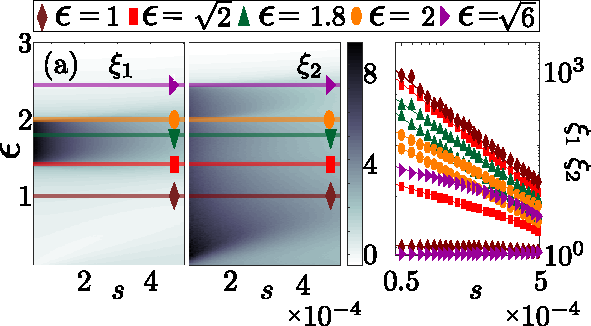
\includegraphics[width=0.5\textwidth]{graphics/loc_length_dipole_BW.pdf}

    \caption{(a) Localization lengths $\xi_1,\,\xi_2$ (color code)  as a function of the energy $\epsilon$ and the disorder strength $s$.
              The localization lengths along each of the black lines are shown in (b).
              The power law exponents $\nu$ of $\xi_1,\,\xi_2$ are
                $\nu\left(\epsilon = 1\right)$ = \{ 0.1006~$\pm$~0.004, 1.96~$\pm$~0.03\}, 
 	        $\nu\left(\epsilon = \sqrt{2}\right)$ = \{ 0.823~$\pm$~0.006, 2.16~$\pm$~0.06\},
 		$\nu\left(\epsilon = 1.8\right)$ = \{ 1.986~$\pm$~0.007, 2.01~$\pm$~0.01\},   
  		$\nu\left(\epsilon = 2\right)$ = \{ 1.428~$\pm$~0.007, 1.376~$\pm$~0.007 \},
 		$\nu\left(\epsilon = \sqrt{6}\right)$ = \{ 0.034~$\pm$~0.002, 0.79~$\pm$~0.01 \}.
	 The atomic position distribution is a Gaussian with width $\sigma$, and the interatomic interaction is a dipole-dipole interaction ($\alpha = 3$) with an interaction strength of $V_0 = 300$.
	     } 
   \label{Fig:2D_loc_length}
\end{figure}  




%
%---------------------------------------------------------------------------------------------------------------------------------------------------------------------------------------
\section{Lieb ladder with correlated disorder}


We observe a ``bending'' of the of the delocalized region of $\xi_1$ (Figure \ref{Fig:2D_loc_length}(a)) towards higher energies $\epsilon>2$, which does not occur for flat disorder.
This bending is caused by the increase of the parameter $s$, which increases the disorder strength and changes the band structure of the disorder-free problem.




%
%\begin{figure}
%
%	      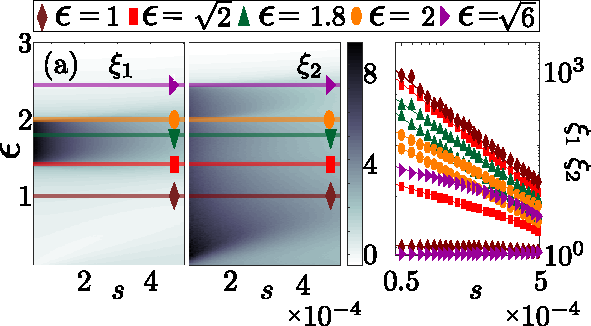
\includegraphics[width=0.5\textwidth]{graphics/loc_length_dipole_BW.pdf}
%
%    \caption{(a) Localization lengths $\xi_1,\,\xi_2$ (color code)  as a function of the energy $\epsilon$ and the disorder strength $s$.
%              The localization lengths along each of the black lines are shown in (b).
%              The power law exponents $\nu$ of $\xi_1,\,\xi_2$ are
%                $\nu\left(\epsilon = 1\right)$ = \{ 0.1006~$\pm$~0.004, 1.96~$\pm$~0.03\}, 
% 	        $\nu\left(\epsilon = \sqrt{2}\right)$ = \{ 0.823~$\pm$~0.006, 2.16~$\pm$~0.06\},
% 		$\nu\left(\epsilon = 1.8\right)$ = \{ 1.986~$\pm$~0.007, 2.01~$\pm$~0.01\},   
%  		$\nu\left(\epsilon = 2\right)$ = \{ 1.428~$\pm$~0.007, 1.376~$\pm$~0.007 \},
% 		$\nu\left(\epsilon = \sqrt{6}\right)$ = \{ 0.034~$\pm$~0.002, 0.79~$\pm$~0.01 \}.
%	 The atomic position distribution is a Gaussian with width $\sigma$, and the interatomic interaction is a dipole-dipole interaction ($\alpha = 3$) with an interaction strength of $V_0 = 300$.
%	     } 
%   \label{Fig:2D_loc_length}
%\end{figure}  



\subsubsection{discuss ``anomalous'' scaling presumably caused by correlations in disorder}
Reference \cite{Leykam2017} gives the power law exponents for various energies
%
\footnote{Power law exponents \cite{Leykam2017}:
$
E = 1:\{\nu_{\xi_1} = 0,\nu_{\xi_2} = 2\}, E = \sqrt 2:\{\nu_{\xi_1} = 2/3,\nu_{\xi_2} = 4/3\},E = 1.8:\{\nu_{\xi_1} = 2,\nu_{\xi_2} = 2\},
E = 2:\{\nu_{\xi_1} = 2/3,\nu_{\xi_2} = 4/3,E = \sqrt 6:\{\nu_{\xi_1} = 0,\nu_{\xi_2} = 2/3\}\}
$.}
for a Lieb ladder with a flat disorder 
potential acting on all lattice sites, which we can reproduce in our setup where the (flat) disorder only acts on intermediate lattice sites.
%
When we apply the experimental disorder to our system, we find an anomalous scaling behavior of the localization lengths
shown in Figure for $E = \sqrt{2}, 2$. In Fig \ref{Fig:2D_loc_length}, we fit the numerical data with the function $f(x) = a \cdot x^\nu$ to obtain the
the power law exponents given in the caption.
For $E = \sqrt 2$ the exponents $\nu_{\xi_1}\approx 1$ and  $\nu_{\xi_2}\approx 2$, while for $E = 2$, the localization lengths $\xi_1$ and $\xi_2$ are parallel (see orange curves) with a
power law exponent $\nu_{\xi_1,\xi_2} \approx 3/2$.
The energies $\epsilon = \sqrt 2, 2$, where the anomalous scaling appears, correspond to the situation where one of the dispersive channels has a band edge with zero group velocity,
while the other dispersive channel 
supports a mid-band state (Figure \ref{Fig:decoupling}(d)).
The difference in the power law exponents between the flat and experimental disorder cannot be 
associated with the fat-tails of the distribution of the $\delta V$, because 
the probability of populating the tails of Eq. \eqref{eq:fattail} is, for the considered parameter regime, approximately zero.
We checked that the anomalous scaling is not caused from the asymmetry of the distribution Eq. \eqref{eq:fattail} around the origin by calculating
the localization length for a flat disorder of the $\delta_V$ which is not centered around the origin.
Using a flat distribution on the atomic position, leading to correlated $\delta_V$, we obtain a very similar scaling behavior of the localization
length shown in Figure \ref{Fig:2D_loc_length}(b).




%
%---------------------------------------------------------------------------------------------------------------------------------------------------------------------------------------
\section{Localized state dynamics}

Reconstructing the localization lengths studied above in an experiment might be challenging. In particular accessing the large localization lengths would require sufficiently large system sizes. On the other hand, one can probe the influence of disorder by initializing the system in a specific state and tracking the subsequent dynamics by measuring the on-site excitation probabilities. Those are probably the most easily accessible observables experimentally using Rydberg atoms by means of fluorescence imaging. The combination of the blockade and facilitation mechanisms together with the single-site addressing offer a unique toolbox for the quantum state preparation. For concreteness lets consider the preparation of the state (XX) [{\bf Ref. to the localized state introduced as a numbered equation in Matteo's part}] localized at rungs $i,i+1$ of the lattice. The state (XX) can then be obtained by application of five pulses on initially all atoms in the ground state as $\ket{\psi_{\rm loc}} = U_1(2 \pi) F_3(\pi) F_2(\frac{\pi}{2}) U_4(\pi) U_1(\frac{\pi}{2}) \ket{\psi_{\rm GS}}$, where $U_j(\theta),F_j(\theta)$ stand for the laser pulse of area $\theta$ in the blockaded ($U$) and facilitated ($F$) regime applied at site $j$ labeling the effective plaquette formed by the four sites corresponding to the $i$-th and $(i+1)$-th rung of the ladder \cite{SM} [{\bf The Supplemental is to be written; then most of this discussion can be probably moved and expanded there and we can only refer in the main text to the SM (??)}]. 

The time evolution is obtained in the usual way as $\ket{\psi(t)} = {\rm exp}[-i H t] \ket{\psi_{\rm loc}}$, where $H$ is the Hamiltonian corresponding to the transfer matrix (\ref{Eq:Transfer_Matrix}) \cite{SM}. In the following we evaluate the probability of excitations $p_i = n_i/\sum_{i=1}^{L} n_i$ at site $i$, where $n_i = \bra{\psi(t)} \hat{n}_i \ket{\psi(t)}$ and
\begin{equation}
	\hat{n}_i =
		\ket{S_{i-1}}\bra{S_{i-1}} + \ket{C_{i}}\bra{C_{i}} + \ket{S_{i}}\bra{S_{i}} + \ket{E_{i}}\bra{E_{i}}
\end{equation}
%\begin{equation}
%	\hat{n}_i = 
%	\begin{cases}
%		\ket{A_{i-1}}\bra{A_{i-1}} + \ket{C_{i}}\bra{C_{i}} + \ket{A_{i}}\bra{A_{i}} + \ket{E_{i}}\bra{E_{i}} \\
%		\text{ upper leg} \\
%		\ket{B_{i-1}}\bra{B_{i-1}} + \ket{D_{i}}\bra{D_{i}} + \ket{B_{i}}\bra{B_{i}} + \ket{E_{i}}\bra{E_{i}} \\
%		\text{ lower leg}
%	\end{cases}
%\end{equation}
is the projector operator on all spin configurations which contain an excitation at site $i$. Here, $S=A$ ($B$) for the upper (lower) leg of the ladder respectively. We then define the average position $\bar{x}$ and the standard deviation $\Delta x$ of the excitations as
\begin{eqnarray}
	\bar{x} &=& \sum p_i i \\
	\Delta x^2 &=& \sum_i p_i i^2 - \bar{x}^2 = \sum_i p_i (i-\bar{x})^2
	\label{eq:Delta x}
\end{eqnarray}

The results of the simulation are shown in Fig. \ref{Fig:time evolution} which shows the evolution of the initial spin configuration, Fig. \ref{Fig:time evolution}a, as a function of a dimensionless time $\tilde{t}$ for a specific value $s=0.01$ in Fig. \ref{Fig:time evolution}b. $\Delta x$, eq. (\ref{eq:Delta x}), at different times $\tilde{t}$ and as a function of $s$ is then shown in Fig. \ref{Fig:time evolution}c. It can be seen that by increasing the disorder strength, the localized state becomes delocalized due to the coupling between the flat and the dispersive bands (hybridization, \cite{Leykam2017}). Increasing further the disorder, it becomes the dominating energy scale which causes the states to localize again. [{\bf Comment on what regime/disorder is achievable in the experiment? Should we try to come up with a specific example to give some numbers? Some extra work - not sure about the parameters for $1/r^3$ interactions.}]

\begin{figure}

	      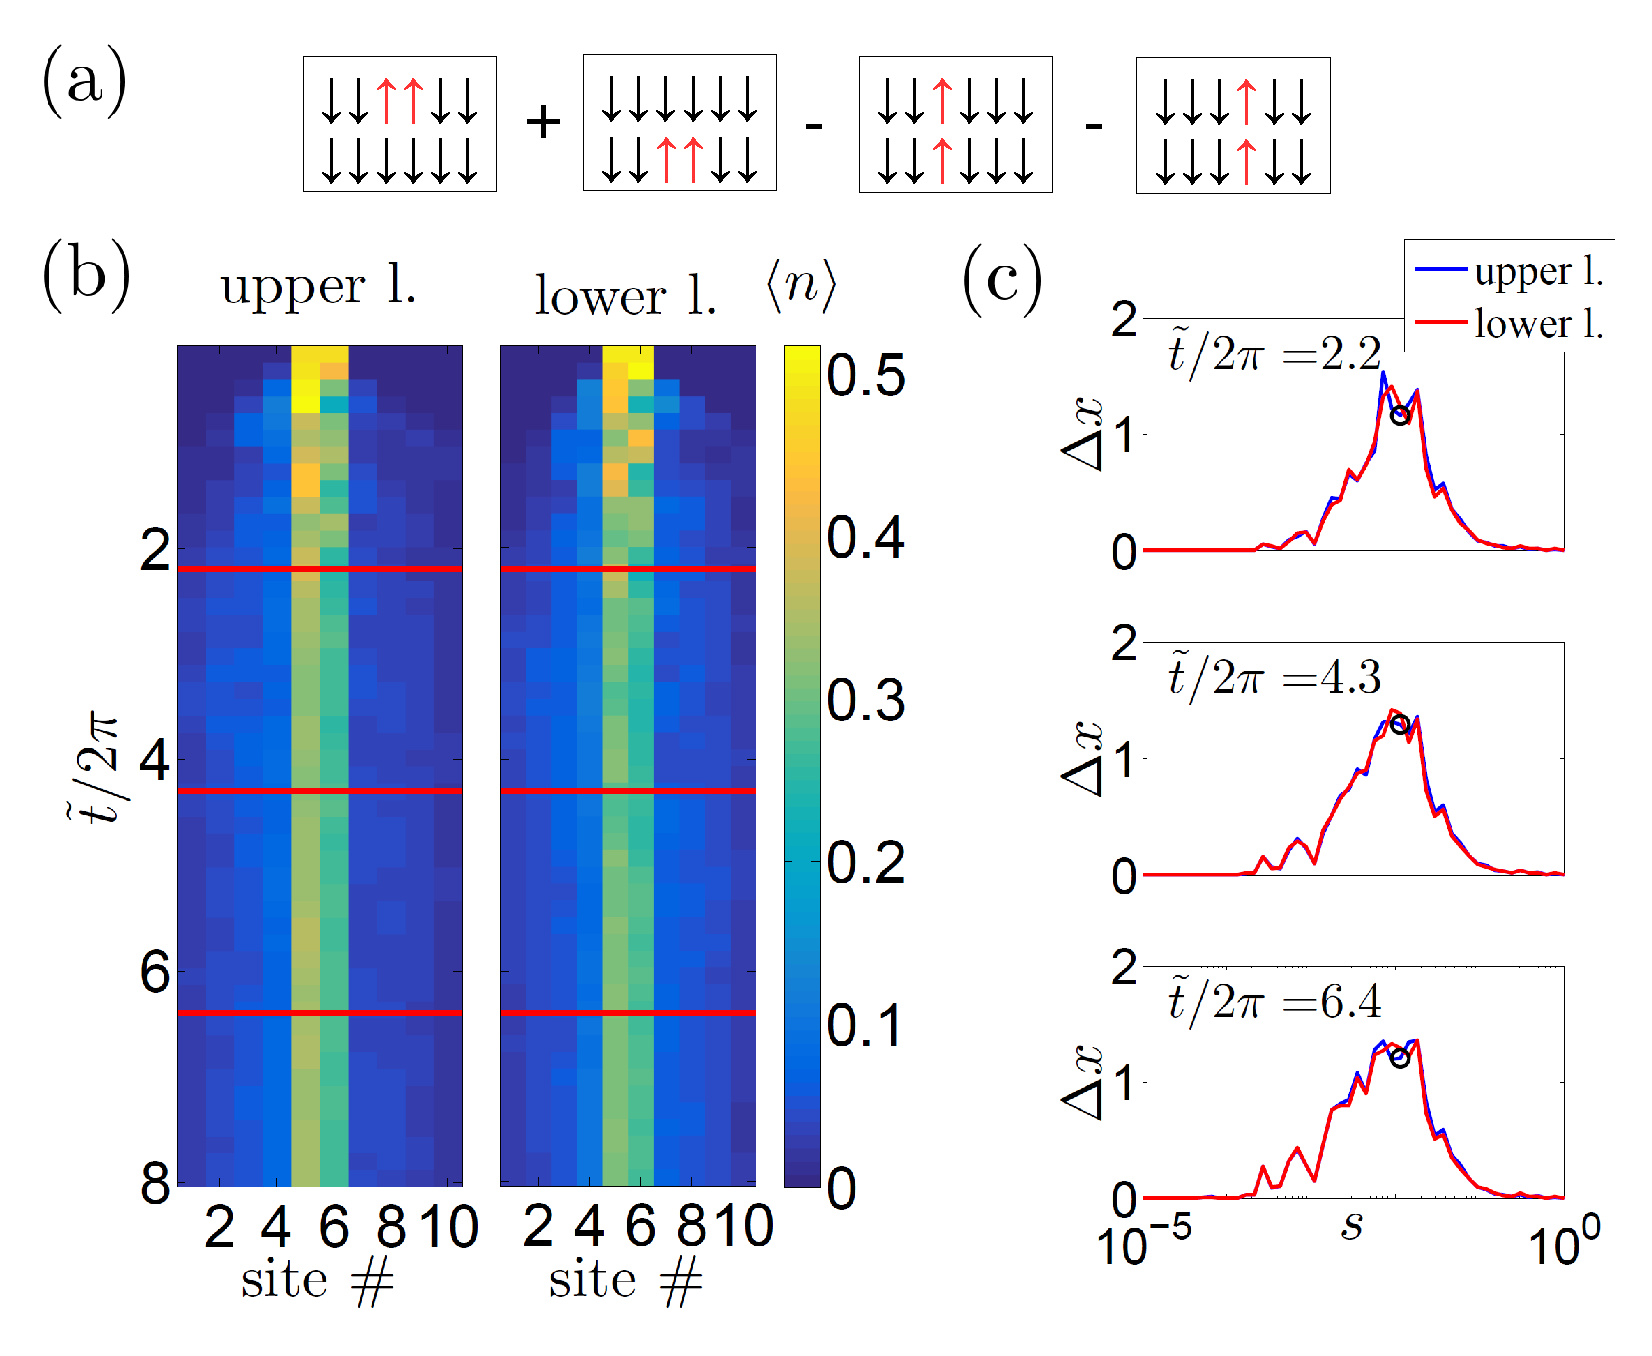
\includegraphics[width=0.5\textwidth]{graphics/time_evolution_CLS_PaperSupport_v2.pdf}
    %
		\caption{(a) Schematic representation of the spin configuration corresponding to the initial localized state. (b) The number of excitations $\av{n}$ given by the time evolution of the localized state with an initial support in the middle (sites 5 and 6) of the ladder of length 10 for $s=0.01$. The left (right) pane shows the time evolution in the upper (lower) leg of the ladder. The horizontal red lines denote three different times for which the respective value of $\Delta x$ is shown as a black circle in (c). (c) Standard deviation of the excitations $\Delta x$ vs. the disorder strength parameter $s$ for three different times. Blue (red) solid lines correspond to upper (lower) leg of the ladder respectively. Results obtained for 1000 disorder realizations.}

 \label{Fig:time evolution}
   
\end{figure}  

\section{Conclusions and Outlook}



%
%---------------------------------------------------------------------------------------------------------------------------------------------------------------------------------------
\section{Supplemental Material}


\subsection{Numerical simulation of the spin dynamics}

[{\bf JM: To be modified.}] \\

We consider the full Hamiltonian
\begin{equation}
	H = \frac{\Omega}{2} \sum_j \sigma^x_j + (-V_0) n_j + V_0 \sum_{j>k} \frac{n_j n_k}{|j-k|^\alpha}
\end{equation}
which we rewrite as dimensionless quantity
\begin{equation}
	H = \sum_j \sigma^x_j + (-\tilde{V}_0) n_j + \tilde{V}_0 \sum_{j>k} \frac{n_j n_k}{|j-k|^\alpha},
\end{equation}
where $\tilde{V}_0 = 2 V_0/\Omega$ (in what follows we label all dimensionless quantities by tilde). This leads to the following effective Hamiltonian on the Lieb lattice of length $L$ expressed in the basis
\begin{equation}
	\mathcal{B}=\{A_1,..,A_L,B_1,..,E_L\}
	\label{eq:basis}
\end{equation}

\begin{equation}
	H_{\rm eff} = H_0 \otimes \mathds{1}_L + H_0^{\rm dis} + \left[ H_1 \otimes G_L + {\rm H.c.} \right],
	\label{eq:H eff}
\end{equation}
where
\begin{equation}
	H_0 =
 \begin{pmatrix}
  	 0 & 0 & 1 & 0 & 0 \\
     0 & 0 & 0 & 1 & 0 \\
     1 & 0 & 0 & 0 & 1 \\
     0 & 1 & 0 & 0 & 1 \\
     0 & 0 & 1 & 1 & 0
 \end{pmatrix},
\end{equation}
$H_1$ is a zero $5 \times 5$ matrix with only non-zero entries $(h_1)_{1,3}=(h_1)_{2,4}=1$, $G_L = \delta_{i,i+1}$ is a $L \times L$ matrix with ones on the first upper diagonal and 
\begin{equation}
	H_0^{\rm dis} = {\rm diag} \left( \tilde{\delta}_{A_1},...,\tilde{\delta}_{A_{L-1}},0,\tilde{\delta}_{B_1},...,\tilde{\delta}_{B_{L-1}},0,\tilde{\delta}_{C_1}=0,...,\tilde{\delta}_{C_{L}}=0,\tilde{\delta}_{D_1}=0,...,\tilde{\delta}_{D_{L}}=0,\tilde{\delta}_{E_1},...,\tilde{\delta}_{E_{L}}\right)
	\label{eq:disorder}
\end{equation}
is a $5L \times 5L$ diagonal disorder matrix, where we impose open boundary conditions by requiring that $\delta_{A_L} = \delta_{B_L}=0$, since spin configurations corresponding to the $A_L,B_L$ basis elements are missing. Analogously we enforce the OBC in the coupling matrix by setting all Hamiltonian elements corresponding to the $L$-th and $2L$-th rows and columns to 0. 

In (\ref{eq:disorder}) the disorder energies $\tilde{\delta}_X$ are generated from first drawing a specific realization of atomic positions at each site of the lattice in all three spatial directions. The realization is drawn from a Gaussian distribution with width $\tilde{\sigma}_\nu$, $\nu=1,2,3$. Furthermore, in order to avoid spurious rare events and motivated by experimental constraints, we impose that only atomic fluctuations $\delta \tilde{x} \leq 1/2, \delta \tilde{y} \leq 1/2$ (i.e. the fluctuations in the plane of the ladder cannot exceed the distance $r_0/2$ from the center of the trap).

We then exactly evolve an initial state
\begin{equation}
	\ket{\psi_0} = \sum_{j=1}^{5L} c_j \ket{b_j},
\end{equation}
where $b_j$ are elements of the basis (\ref{eq:basis}) [strictly speaking there are only $5L-2$ non-trivial elements due to the OBC]. 




\bibliographystyle{apsrev4-1}

\bibliography{bibliography}


\end{document}